%%% LaTeX Template: Article/Thesis/etc. with colored headings and special fonts
%%%
%%% Source: http://www.howtotex.com/
%%% Feel free to distribute this template, but please keep to referal to http://www.howtotex.com/ here.
%%% February 2011
%%%
%%% Last updated January 2018 by CDM

%%%  Preamble
\documentclass[11pt,letterpaper]{article}
\usepackage[margin=1.0in]{geometry}
\usepackage[T1]{fontenc}
\usepackage[bitstream-charter]{mathdesign}
\usepackage[latin1]{inputenc}					
\usepackage{amsmath}						
\usepackage{xcolor}
\usepackage{cite}
\usepackage{hyphenat}
\usepackage{graphicx}
\usepackage{float}
\usepackage{subfigure}
\usepackage{sectsty}
\usepackage[compact]{titlesec} 
\usepackage[tablegrid]{vhistory}
\usepackage{url}


\allsectionsfont{\color{accentcolor}\scshape\selectfont}

%%% Definitions
\definecolor{accentcolor}{rgb}{0.0,0.0,0.5} 
\newcommand{\teamname}{The Brew Crew}
\newcommand{\productname}{Beverage Management}
\newcommand{\coursename}{CSE 4316: Senior Design I}
\newcommand{\semester}{Summer 2020}
\newcommand{\docname}{Project Charter}
\newcommand{\department}{Department of Computer Science \& Engineering}
\newcommand{\university}{The University of Texas at Arlington}
\newcommand{\authors}{Bishal Paudel \\ Nirjal Phaiju \\ Sima Raymajhi \\ Lokendra B. Chhetri \\ Kunal Samant }

%%% Headers and footers
\usepackage{fancyhdr}
	\pagestyle{fancy}						% Enabling the custom headers/footers
\usepackage{lastpage}	
	% Header (empty)
	\lhead{}
	\chead{}
	\rhead{}
	% Footer
	\lfoot{\footnotesize \teamname \ - \semester}
	\cfoot{}
	\rfoot{\footnotesize page \thepage\ of \pageref{LastPage}}	% "Page 1 of 2"
	\renewcommand{\headrulewidth}{0.0pt}
	\renewcommand{\footrulewidth}{0.4pt}

%%% Change the abstract environment
\usepackage[runin]{abstract}			% runin option for a run-in title
%\setlength\absleftindent{30pt}			% left margin
%\setlength\absrightindent{30pt}		% right margin
\abslabeldelim{\quad}	
\setlength{\abstitleskip}{-10pt}
\renewcommand{\abstractname}{}
\renewcommand{\abstracttextfont}{\color{accentcolor} \small \slshape}	% slanted text

%%% Start of the document
\begin{document}

%%% Cover sheet
{\centering \huge \color{accentcolor} \sc \textbf{\department \\ \university} \par}
\vspace{1 in}
{\centering \huge \color{accentcolor} \sc \textbf{\docname \\ \coursename \\ \semester} \par}
\vspace{0.5 in}
\begin{figure}[h!]
	\centering
   	
\includegraphics[width=0.40\textwidth]{images/beverage}
\end{figure}
\vspace{0.5 in}
{\centering \huge \color{accentcolor} \sc \textbf{\teamname \\ \productname} \par}
\vspace{0.5 in}
{\centering \large \sc \textbf{\authors} \par}
\newpage


%\vspace{1 in}
%\centerline{January 13th, 2012}
%\newpage

%%% Revision History
\begin{versionhistory}
	  \vhEntry{0.1}{07.30.2020}{BP}{document creation}
	  \vhEntry{0.2}{07.09.2020}{BP}{section 1 added}
	  \vhEntry{0.3}{08.03.2020}{LC}{Section 2,3,6,7,8,9 (missing)}
	  \vhEntry{0.4}{08.03.2020}{LC}{sections 4 and 5 added}
\end{versionhistory}
\newpage

%%% Table of contents
\setcounter{tocdepth}{2}
\tableofcontents
\newpage

%%% List of figures and tables (optional)
\listoffigures
%\listoftables
\newpage

\section{Product Concept}
This section describes the purpose, use and intended user audience for the Beverage Management app. Beverage Management app is an android application that provides an efficient way to manage large collection of beverages using smartphone.

\subsection{Purpose and Use}
Beverage Management is an android application that works as a virtual inventory and allows user to effectively manage and keep track of several beverages. Users can use this app to keep track of name, storage location, brewery, style, volume, manufactured date and best before date. It also allows user to search and sort the beverages according to the date, style etc.

\subsection{Intended Audience}
The intended audience for this application are those people who have large collection of beverages in their home and are looking for easy ways to manage them free of cost. It can also be used in local grocery stores, bars and restaurants to keep track of their beverage inventory. Our app is intended for general use but it can certainly be expanded into a more complex inventory management system with additional features.  

\begin{figure}[h!]
	\centering
   	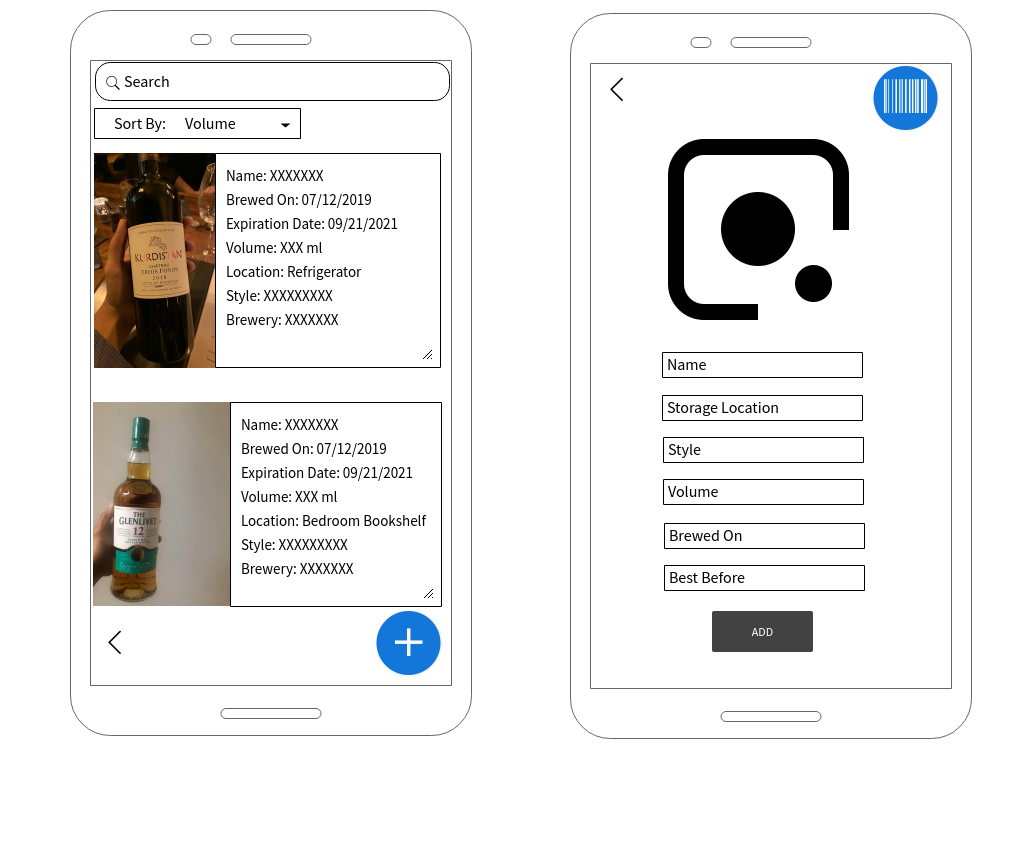
\includegraphics[width=0.60\textwidth]{images/CD.png}
    \caption{ conceptual drawing of Beverage Management App (Home screen and Add screen) }
\end{figure}

\newpage
\section{Product Description}
This section provides a description of your product and defines it's primary features and functions. The purpose is to give the document reader/reviewer enough information about the product to allow them to easily follow the specification of requirements found in the remainder of the document. Your header for this section should introduce the section with a brief statement such as: "This section provides the reader with an overview of X. The primary operational aspects of the product, from the perspective of end users, maintainers and administrators, are defined here. The key features and functions found in the product, as well as critical user interactions and user interfaces are described in detail." Using words, and pictures or graphics where possible, specify the following:

\subsection{Features \& Functions}
What the product does and does not do. Specify in words what it looks like, referring to a conceptual diagram/graphic (Figure X).  Define the principle parts/components of the product. Specify the elements in the diagram/graphic that are part(s) of this product as well as any associated external elements (e.g., the Internet, an external web server, a GPS satellite, etc.)

\subsection{External Inputs \& Outputs}
Describe critical external data flows. What does your product require/expect to receive from end users or external systems (inputs), and what is expected to be created by your product for consumption by end users or external systems (outputs)? In other words, specify here all data/information to flow into and out of your systems. A table works best here, with rows for each critical data element, and columns for name, description and use.

\subsection{Product Interfaces}
Specify what all operational (visible) interfaces look like to your end-user, administrator, maintainer, etc. Show sample/mocked-up screen shots, graphics of buttons, panels, etc. Refer to the critical external inputs and outputs described in the paragraph above.

\newpage
\section{Customer Requirements}
Here, we have requirements that our group came up with after having a detailed conversation with our customer and group members. These requirements are documentation of what our customer expects from our mobile application and these requirements will not be changed without the consent of the customer. 

\subsection{Accurate Inventory Tracking}
\subsubsection{Description}
Customers shall be able to track the total number of a specific beer available in their inventory.
\subsubsection{Source}
Nirjal
\subsubsection{Constraints}
N/A
\subsubsection{Standards}
N/A
\subsubsection{Priority}
High

\subsection{An Attractive and easy to use User Interface}
\subsubsection{Description}
Customers shall be able to navigate through our application without any confusion and complications.
\subsubsection{Source}
Kunal
\subsubsection{Constraints}
N/A
\subsubsection{Standards}
N/A
\subsubsection{Priority}
High

\subsection{Successful access to the Camera}
\subsubsection{Description}
The application shall have no problem using the user’s cellphone camera after getting user’s consent.
\subsubsection{Source}
Kunal
\subsubsection{Constraints}
The user will have to put in the extra work in order to enter the product name and categorize it manually if the camera is not functioning properly.
\subsubsection{Standards}
N/A
\subsubsection{Priority}
Critical

\subsection{Login Functionality}
\subsubsection{Description}
The user shall be able to login to their account without any complications with correct username and password. In case user forgets the password, there shall be a way for the user to recover it.
\subsubsection{Source}
Lokendra
\subsubsection{Constraints}
N/A
\subsubsection{Standards}
N/A
\subsubsection{Priority}
Critical

\subsection{Search by Product Name, Brewery, and Beer style}
\subsubsection{Description}
The application shall be able to search and display the product that already exists in the inventory on the basis of product name, brewery, and beer style.
\subsubsection{Source}
Sima and Chris
\subsubsection{Constraints}
N/A
\subsubsection{Standards}
N/A
\subsubsection{Priority}
Critical

\subsection{Notification if the beer is nearing expiry date}
\subsubsection{Description}
The application shall notify the user about the products in the inventory that are nearing their best by date.
\subsubsection{Source}
Chris
\subsubsection{Constraints}
N/A
\subsubsection{Standards}
N/A
\subsubsection{Priority}
Critical

\subsection{Sort by best by date, brew date, and format}
\subsubsection{Description}
The application shall be able to sort the displayed items based on nearest expiration date, brew date and item size (12 oz. bottle, 12 oz. can, .33 L bottle, etc.).
\subsubsection{Source}
Chris
\subsubsection{Constraints}
N/A
\subsubsection{Standards}
N/A
\subsubsection{Priority}
High

\subsection{Create a Storage Location with NxM rows and columns}
\subsubsection{Description}
The application shall be able to create and save a storage location in the format of NxM rows and columns 
\subsubsection{Source}
Chris
\subsubsection{Constraints}
N/A
\subsubsection{Standards}
N/A
\subsubsection{Priority}
High

\subsection{Ability to take a picture of bottle/can to store that}
\subsubsection{Description}
The application shall allow user to click and save a photo of the item that we are storing.
\subsubsection{Source}
Chris
\subsubsection{Constraints}
N/A
\subsubsection{Standards}
N/A
\subsubsection{Priority}
Moderate

\subsection{Notes section to add any comments that user may find useful(example: Tasting Notes)}
\subsubsection{Description}
The application shall allow user to click and save a photo of the item that we are storing.
\subsubsection{Source}
Chris
\subsubsection{Constraints}
N/A
\subsubsection{Standards}
N/A
\subsubsection{Priority}
Low

\subsection{Warning when mobile storage space is low}
\subsubsection{Description}
The application shall warn users when mobile storage space is low cannot be to save photos, notes, etc.
\subsubsection{Source}
Bishal
\subsubsection{Constraints}
N/A
\subsubsection{Standards}
N/A
\subsubsection{Priority}
Low
\newpage
\section{Packaging Requirements}
The application software shall be loaded to our client's (Dr. Conly) mobile device. The client's preferred platform shall be android OS. Client/User can also download via google play store for free. Additionally, the application software shall be stored on team lead's external hard drive and GitHub repository.  

\subsection{Installing Application}
\subsubsection{Description}
The application will be installed in the client's device by private downloadable link provided by the team, the initial setup or installation must be required by the user.   
\subsubsection{Source}
Team
\subsubsection{Constraints}
User must have access to internet connectivity. 
\subsubsection{Standards}
N/A
\subsubsection{Priority}
High
\newpage
\section{Performance Requirements}
Include a header paragraph specific to your product here. Performance requirements address items such as: how fast specific critical operations must complete; how long it takes to start/stop activities; how long the battery must last; maximum time it must take to set up; etc.

\subsection{Requirement Name}
\subsubsection{Description}
Detailed requirement description...
\subsubsection{Source}
Source
\subsubsection{Constraints}
Detailed description of applicable constraints...
\subsubsection{Standards}
List of applicable standards
\subsubsection{Priority}
Priority
\newpage
\section{Safety Requirements}
Include a header paragraph specific to your product here. Safety requirements might address items specific to your product such as: no exposure to toxic chemicals; lack of sharp edges that could harm a user; no breakable glass in the enclosure; no direct eye exposure to infrared/laser beams; packaging/grounding of electrical connections to avoid shock; etc.

\subsection{Requirement Name}
\subsubsection{Description}
Detailed requirement description...
\subsubsection{Source}
Source
\subsubsection{Constraints}
Detailed description of applicable constraints...
\subsubsection{Standards}
List of applicable standards
\subsubsection{Priority}
Priority
\newpage
\section{Maintenance \& Support Requirements}
Include a header paragraph specific to your product here. Maintenance and support requirements address items specific to the ongoing maintenance and support of your product after delivery. Think of these requirements as if you were the ones who would be responsible for caring for customers/end user after the product is delivered in its final form and in use "in the field". What would you require to do this job? Specify items such as: where, how and who must be able to maintain the product to correct errors, hardware failures, etc.; required support/troubleshooting manuals/guides; availability/documentation of source code; related technical documentation that must be available for maintainers; specific/unique tools required for maintenance; specific software/environment required for maintenance; etc.

\subsection{Requirement Name}
\subsubsection{Description}
Detailed requirement description...
\subsubsection{Source}
Source
\subsubsection{Constraints}
Detailed description of applicable constraints...
\subsubsection{Standards}
List of applicable standards
\subsubsection{Priority}
Priority
\newpage
\section{Other Requirements}
Include a header paragraph specific to your product here. In this section specify anything else that is required for the product to be deemed complete. Include requirements related to customer setup and configuration if not specified in a previous requirement. Add any known requirements related to product architecture/design, such as modularity, extensibility (for future enhancements), or adaptation for a specific programming language. Consider requirements such as portability of your source code to various platforms (Windows, Linux, Unix Mac OS, etc.).

\subsection{Requirement Name}
\subsubsection{Description}
Detailed requirement description...
\subsubsection{Source}
Source
\subsubsection{Constraints}
Detailed description of applicable constraints...
\subsubsection{Standards}
List of applicable standards
\subsubsection{Priority}
Priority
\newpage
\section{Future Items}
In this last section, you will reiterate all requirements that are listed as priority 5. This is repetitive, but necessary as a concise statement of features/functions that were considered/discussed and documented herein, but will NOT be addressed in the prototype version of the product due to constraints of budget, time, skills, technology, feasibility analysis, etc. Use the following format for this section.

\subsection{Requirement Name}
\subsubsection{Description}
Detailed requirement description...
\subsubsection{Source}
Source
\subsubsection{Constraints}
Detailed description of applicable constraints...
\subsubsection{Standards}
List of applicable standards
\subsubsection{Priority}
Priority
\newpage

%%% References
\bibliographystyle{plain}
\bibliographystyle{reference/IEEEtran_custom}
\bibliography{reference/refs}{}

\end{document}